\chapter{Dataset}\label{chap:dataset}

For our experiments, we make use of a dataset composed of Reber sequences. A Reber sequence is a grammar string made of finite states, in simple words, formed by using a confined set of characters. In the research paper that proposed the LSTM \cite{lstm}, the authors use embedded Reber grammar due to its short time lags. For our purpose, we use a simple version of this embedded Reber grammar, called Reber grammar (\cite{reber}).

The following figure shows the flow diagram to generate Reber grammar sequences:

\begin{figure}[h]
    \centering
    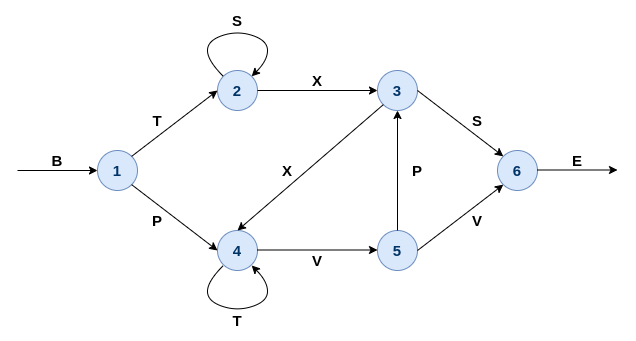
\includegraphics[width=0.9\linewidth]{images/dataset/reber.png}
    \caption[Flow diagram to generate Reber grammar sequences]{Flow diagram to generate Reber grammar sequences}
    \label{fig:reber}
\end{figure}

As shown in the above graph, a sequence is a true Reber sequence if
\begin{enumerate}
    \item it contains only these characters: \textit{B, E, P, S, T, V, X}
    \item it starts with a $B$ and ends with an $E$, \textit{always!}
    \item it strictly follows the transition diagram shown in figure \ref{fig:reber}.
\end{enumerate}

After starting at $B$, we move from one node to the next until we reach $E$. If we have more than one path to choose from, we can randomly select one of them. Two of the allowed characters, $S$ and $T$, have a self-loop at nodes $2$ and $4$, respectively, meaning we can have more than two consecutive $S$s and $T$s. For example, the following table shows some of the true and false Reber sequences from our dataset:

\begin{table}[h]
	\centering
	\begin{tabular}{|c|c|}
	    \hline
		\textbf{True Reber sequences} & \textbf{False Reber sequences} \\
		\hline
		BPTVPXTTVVE & BTTVPXTVPSE \\
		BTSXXTTTTVVE & BPSXXTTTVPSE \\
		BTSSXXTTVVE & BPSSSXXTVVE \\
		BTXXVPXTVVE & BTTTVPXTVVE \\
		BPTTTTTVPSE & BPSSXXTTVVE \\
		\hline
	\end{tabular}
	\caption[A few examples of true and false Reber sequences]{A few examples of true and false Reber sequences.}
	\label{tab:reber}
\end{table}

Since, to our knowledge, there is no public dataset of Reber sequences available, we created our own dataset of $25000$ true and false Reber sequences combined. We follow the same flow, as shown in figure \ref{fig:reber}, to generate true Reber sequences. Then, by slightly altering the same procedure, we generate false Reber sequences.

We then split this dataset into a train-test set, details of which are shown in the following bar chart:

\begin{figure}[h]
    \centering
    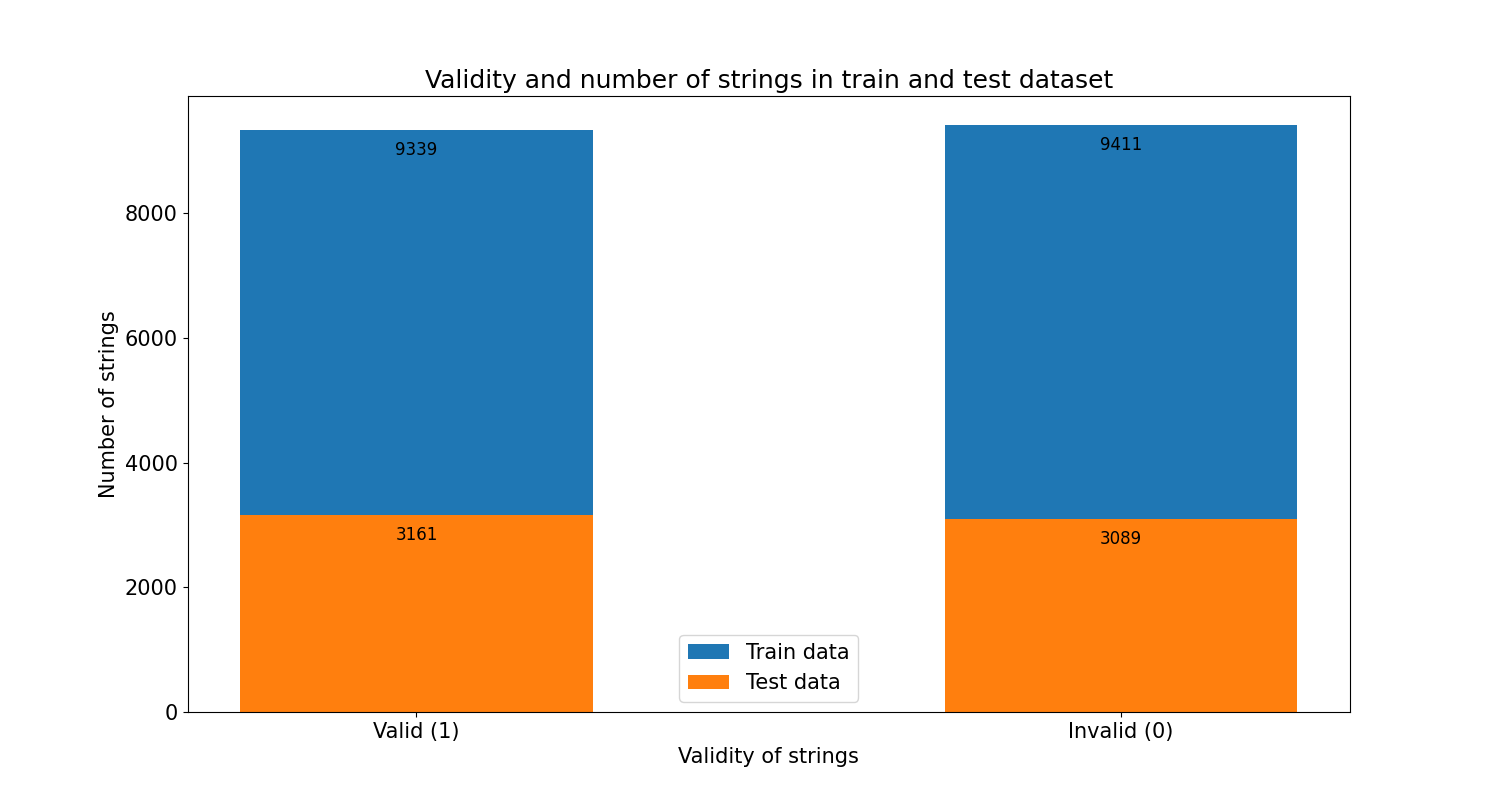
\includegraphics[width=1.0\linewidth]{images/dataset/string_counts.png}
    \caption[Validity and number of strings in train-test dataset]{Number of valid (true) and invalid (false) Reber sequences in our train-test set}
    \label{fig:string_count}
\end{figure}

Our dataset has $12500$ true Reber sequences and $12500$ false, thus totaling $25000$. Although the true Reber sequences only contain allowed characters (i.e., \textit{B, E, P, S, T, V, X}), the false sequences may contain any character from A to Z.

Out of $25000$ total sequences, our train-test set contains $18750$ and $6250$ sequences, respectively. Furthermore, this train-test individually include the following number of true and false Reber sequences:

\begin{table}[h]
	\centering
	\begin{tabular}{|c|c|c|}
	    \hline
		 & \textbf{Training set} & \textbf{Test set} \\
		\hline
		\textbf{Valid (true)} & 9339 & 3161 \\
		\textbf{Invalid (false)} & 9411 & 3089 \\
		\hline
	\end{tabular}
	\caption[The number of true and false Reber sequences in our train-test set]{The number of true and false Reber sequences in our train-test set.}
	\label{tab:train-test_strings}
\end{table}
Next, we visualize the string length distribution that shows not only the minimum and maximum string length but also the number of strings for each length value.

The following plot displays the string length distribution of our entire dataset:

\begin{figure}[h]
    \centering
    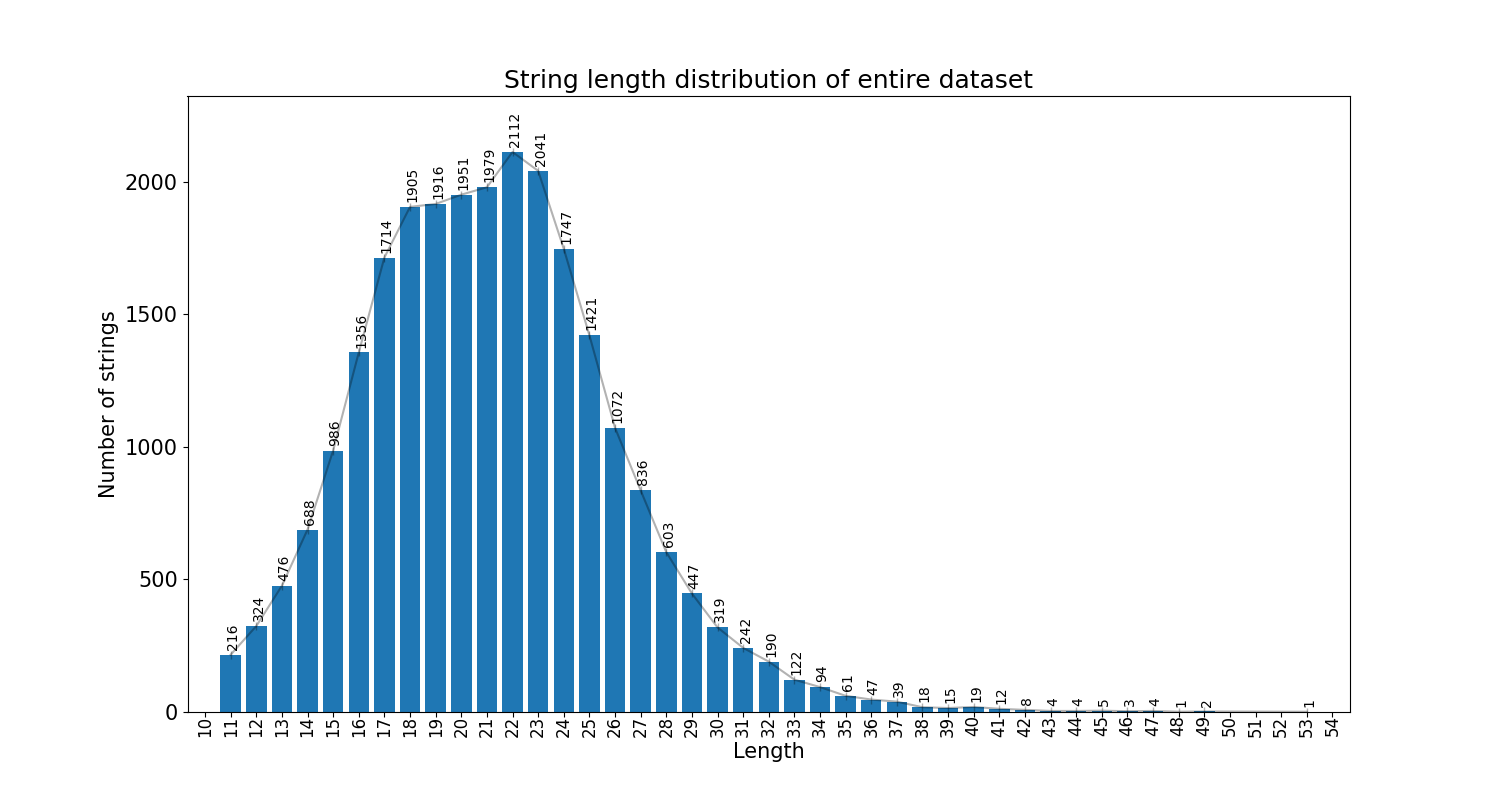
\includegraphics[width=0.9\linewidth]{images/dataset/entire_dataset_string_len.png}
    \caption[String length distribution of entire dataset]{String length distribution of entire dataset}
    \label{fig:string_len}
\end{figure}

As we can see in the above plot, in our entire dataset, the minimum string length is $11$ with $216$ sequences, and the maximum string length is $53$ with $1$ sequence. The highest number of strings, $2112$ strings, in our entire dataset is of length $22$.

The following plot displays the string length distribution of our train dataset:

\begin{figure}[h]
    \centering
    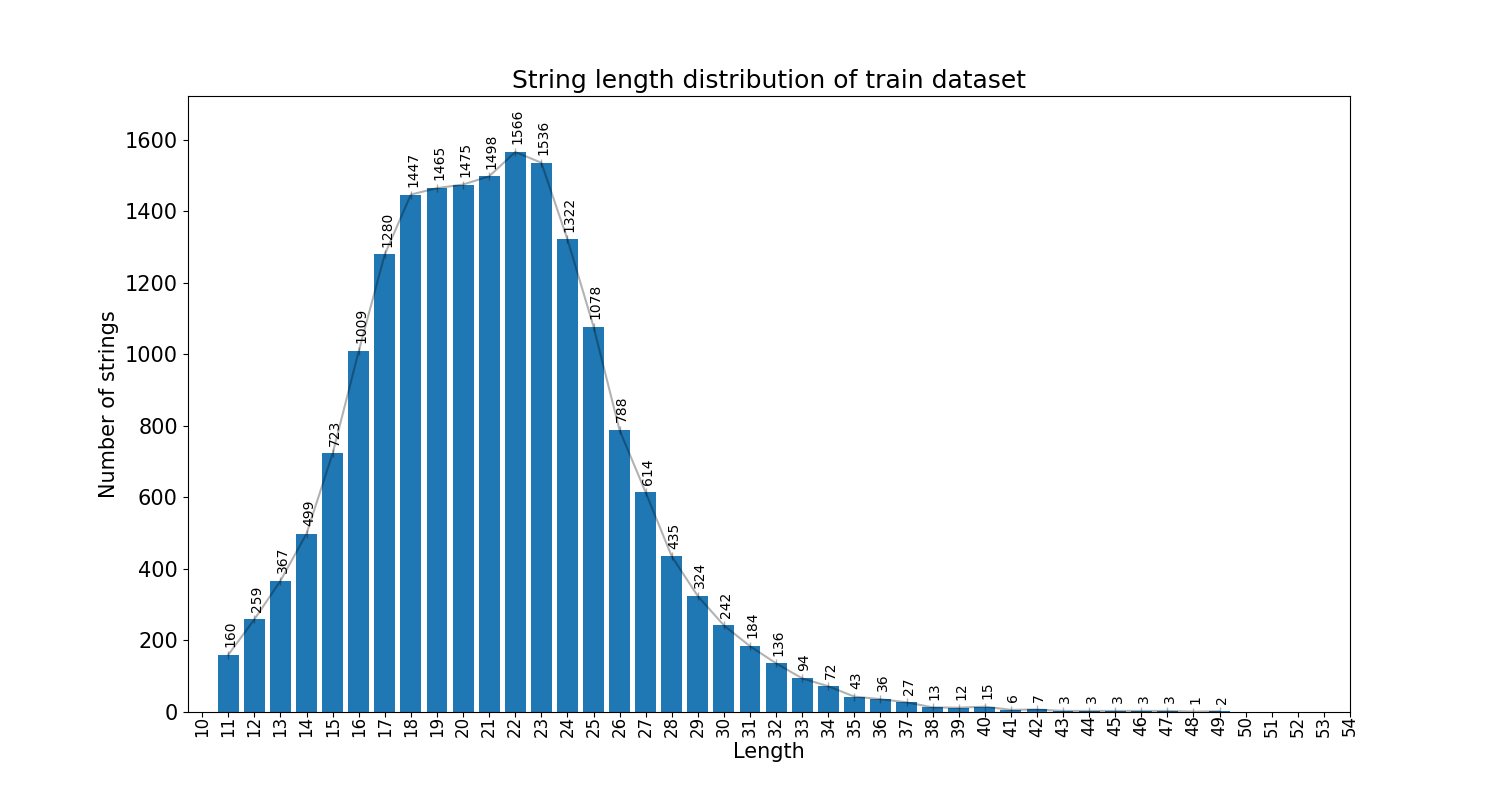
\includegraphics[width=0.9\linewidth]{images/dataset/train_dataset_string_len.png}
    \caption[String length distribution of train dataset]{String length distribution of train dataset}
    \label{fig:train_string_len}
\end{figure}

As we can see in the above plot, in our train dataset, the minimum string length is $11$ with $160$ sequences, and the maximum string length is $49$ with $2$ sequence. The highest number of strings, $1566$ strings, in our train dataset is of length $22$.

The following plot displays the string length distribution of our test dataset:

\begin{figure}[h]
    \centering
    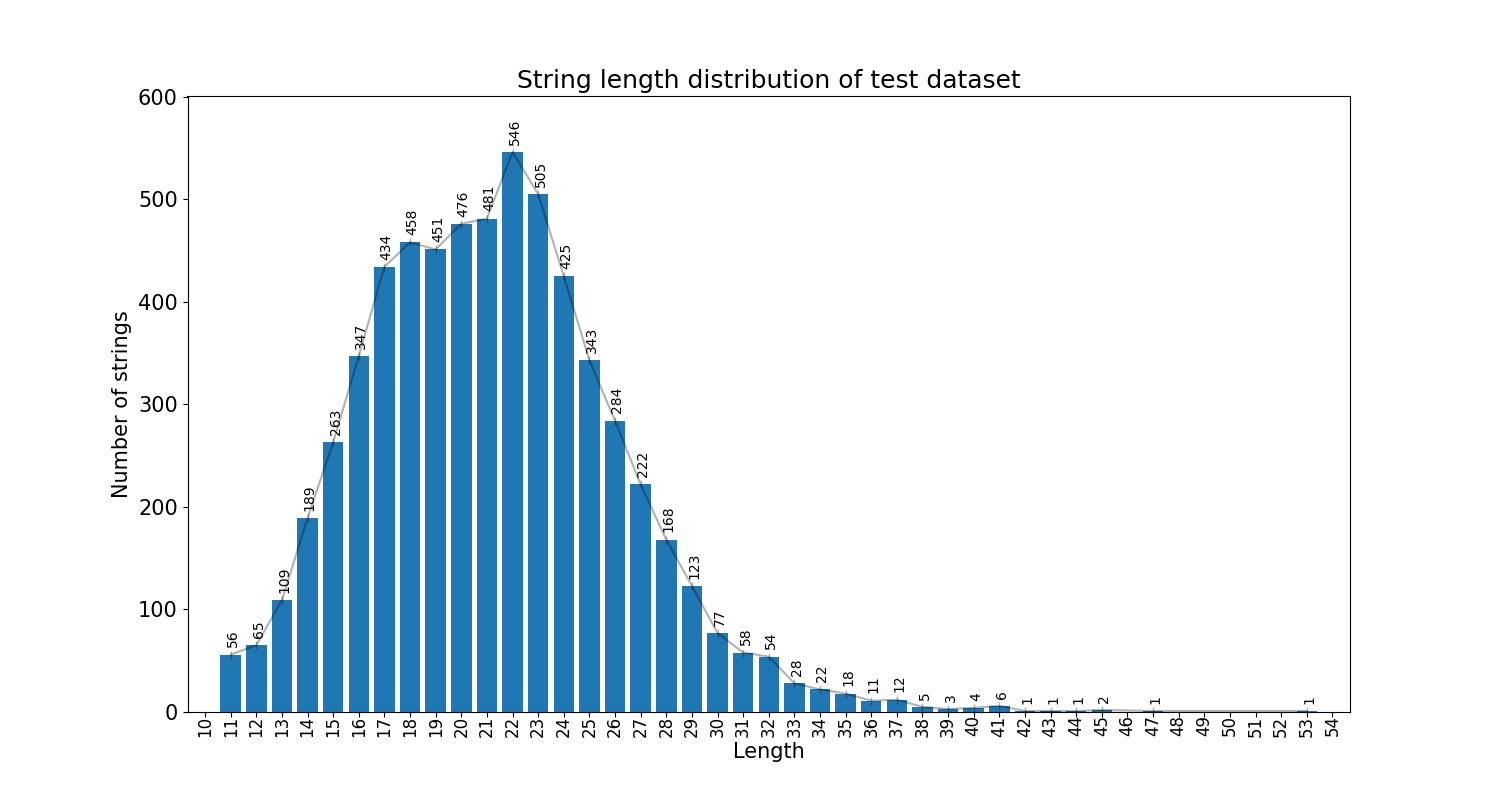
\includegraphics[width=0.9\linewidth]{images/dataset/test_dataset_string_len.png}
    \caption[String length distribution of test dataset]{String length distribution of test dataset}
    \label{fig:test_string_len}
\end{figure}

As we can see in the above plot, in our test dataset, the minimum string length is $11$ with $56$ sequences, and the maximum string length is $53$ with $1$ sequence. The highest number of strings, $546$ strings, in our test dataset is of length $22$.